\chapter{Complementos de Scrum}

Rodeando el núcleo de Scrum se encuentra un anillo de complementos. Estos complementos son métodos y técnicas complementarias a Scrum, sujerencias y recomendaciones, lecciones aprendidas y conceptos aledaños. En este capítulos trataremos estos temas.

% Malas prácticas, consejos, tecnicas complementarias, casos de estudios

%Técnicas para requerimientos
% Historias de usuarios
% Técnica Killen 
% Mapas de historia
%Técnicas de Planeación
%Técnicas de estimación
% Poker de planeación
%Técnicas de Comunicación
% Radiadores de información
% Scrum task board
% Comunicación osmótica

\newpage
\section{Técnicas para requerimientos}

\subsection{Historias de usuarios}

Para Scrum las hipótesis de requerimientos se representan en items de Backlog de producto PBI. A estos PBIs se los suele denominar "Story" o "Historias de Usuarios"\footnote{Las "User Story" son una técnica de eXtremme Programming (XP)}. El Product Backlog incluye incisos o Stories que aportan valor al cliente y que suelen ser descripción de requisitos funcionales. Aunque también puede incluir entradas para exploración de características, necesidades del cliente u opciones técnicas, requerimientos no funcionales, el trabajo necesario para lanzar el producto, y otros incisos, así como la configuración del entorno o arreglar defectos \footnote{\cite{Scrum-Institute-2015}}. O sea que puede proporcionar valor en forma indirecta mediante el aumento de la calidad o la reducción de los incidentes en el largo plazo \footnote{\cite{Scrum-Institute-2015}}.

Las historias representan un concepto verificable y simple, que el Product Owner quiere implementar en el producto. Según el concepto general de metodología Ágil, la historia se define como una "promesa de una conversación" o una "descripción de una característica" \footnote{\cite{UNTREF-2014}, \cite{Dan-North-2015}}. Según esta perspectiva, la historias de usuario representa una "funcionalidad de aplicación" para un usuario y que brinda un beneficio (ROL + FUNCIONALIDAD + BENEFICIO). Las mismas se escriben siempre con lenguaje de negocio y respetando la siguiente pauta de estructura:

\textbf{COMO} <ROL> \textbf{QUIERO} <FUNCIONALIDAD> \textbf{PARA QUE} <BENEFICIO>

Por ejemplo:

COMO ScrumMaster QUIERO que las reuniones no se extiendan más de un tiempo consensuado PARA QUE no se pierda el foco.

La historia de usuario no es exactamemte un requerimiento, pero puede considerarse como el título de una hipótesis de requerimiento como recordatorio de algo relevante a conversar con el usuario o cliente. En consecuencia lo relevante es su evolución como conversación \footnote{\cite{UNTREF-2014}}.

La historia de usuario describe lo que el usuario quiere hacer desde la perspectiva de una interacción con un proceso de negocio, describe el objetivo del usuario en términos de necesidad de obtener algo que se hace en el negocio \footnote{\cite{Scott-Bellware-2008}}.

Según Dan North y en el marco de Behavior-Driven Development (BDD), una Story es más un requerimiento, pues tiene que ser una descripción de un requisito y su beneficio para el negocio, y un conjunto de criterios con los que todos estamos de acuerdo de qué es o lo que se hace, "lo que el cliente necesita" \footnote{\cite{Dan-North-2015}}. 

\subsubsection{Criterio de demarcación}

Existen ciertas características a tener en cuenta a la hora de escribir una historia de usuario y determinar cuál es una válida. El criterio de demarcación aceptado en metodología ágil en general es el criterio INVEST que consta de seis características a cumplir \footnote{\cite{UNTREF-2014}, \cite{Scrum-Alliance-2015}}:

\begin{enumerate}

\item \textbf{Independiente:} debe ser atómica.

\item \textbf{Negociable:} debe ser conversable y en consecuencia negociable (es viva).

\item \textbf{Valueble:} debe generar un valor al usuario o cliente. Una Story sin una declaración de la motivación del usuario a menudo se piensa que es no accionable; es decir, la historia no se puede estimar o implementar fácilmente \footnote{\cite{Scott-Bellware-2008}}.

\item \textbf{Estimable:} se debe poder estimar.

\item \textbf{Pequeña:} debe ser lo suficientemente pequeña para entrar en un sprint o iteración. El tamaño pequeño de las historias ayuda a reducir el tamaño del lote, a incrementar el flujo de valor hacia el cliente y a asegurar que cada miembro del equipo de desarrollo pueda hacer una contribución valiosa cada día. Por ejemplo en cada Sprint se pueden completar entre cuatro y ocho historias pequeñas.

\item \textbf{Probable:} debe poder permitir la contrastabilidad. La contrastabilidad del enunciado de la historia es la propiedad de ésta de ser capaz de ser sometida a una prueba empírica a fin de evaluar su adecuación o no a los hechos a los que se refiere o resultados esperados. Esta característica es crucial para hacer ingeniería, sin la contrastabilidad no se hace ingeniería.

\end{enumerate}

\subsubsection{¿Qué NO es una Historia de Usuario?}

Si no cumple con el criterio INVEST es bastante probable que no sea una Story. Por ejemplo una tarea puramente técnica (que le interesa solo al desarrollador), un refactoring técnico o un Spike no cumplen con INVEST y en su generalidad no son Story. Veamos:

\begin{itemize}

\item \textbf{Spike:}
No es una Story ya que es una tarea de investigación y/o experimentación en formato time-boxing por lo que no cumple con ser testeable ni estimable (no cumple con dos criterios).

\item \textbf{Refactoring Task:}
Es una tarea técnica que no es valuable o su valoración es a futuro o en relación a un atributo de calidad que puede no estar directamente solicitado por el cliente o no impacta en beneficio inmediato para el cliente, ya que podría estar resolviendo una deuda técnica. Esto no quiere decir que no pueda haber una "story de refactoring" que puede proporcionar valor en forma indirecta mediante el "aumento de la calidad o la reducción de los incidentes en el largo plazo".

\item \textbf{Technical Story:}
“Cada historia tiene que ser valorada por los usuarios. Pero eso sería un error."\footnote{\cite{Cohn-2004}} Pues en realidad, una historia de usuario describe la funcionalidad que será valiosa para un usuario o comprador de un sistema o software \footnote{\cite{Cohn-2004}}. Hay historias que especifican aspectos técnicos que no son valiosos para el usuario sino mas bien para el cliente o comprador (la valoración es transitiva y no directa). Historias técnicas pueden ser valorados por los compradores que contemplan la compra del producto, pero no serían valorados por los usuarios reales. Pero esto no es lo que podemos llamar una "Technical Story" sino que es una Story con aspectos técnicos que tiene valor para el cliente. Para Scott Ambler en Agile Modeling, una Story es una definición de muy alto nivel de un requerimiento que puede ser funcional o no, por ejemplo de un requerimiento técnico \footnote{\cite{Scott-Ambler-2015}}, por ejemplo: "como usuario quiero que las transcripciones estén disponibles en línea a través de un navegador estándar lo que me permite acceder desde cualquier lugar"\footnote{\cite{Scott-Ambler-2015}}.

Cuando se habla de "Technical Story" se referencia a aquella historia técnica que sólo es valorada por los desarrolladores. Estas historias son las que se quieren evitar y considerar como Technical Story que podría ser una tarea técnica o una historia mejor redactada. Este tipo de historias se centran en la tecnología y las ventajas para los programadores. Es muy posible que las ideas detrás de estas historias sean buenas, pero en cambio deben ser escritas para que los beneficios a los clientes o usuarios sean evidentes. Esto permitirá que el cliente priorizar inteligentemente estas historias en el calendario de desarrollo \footnote{\cite{Cohn-2004}}.

Para la Agile Alliance una Story no se corresponden en general a un "componente técnico" o de la "interfaz de usuario", pues a pesar de que a veces puede ser un atajo útil hablar de por ejemplo "la historia de diálogo de búsqueda", pantallas, cuadros de diálogo y botones, no son historias de usuario \footnote{\cite{Scrum-Alliance-2015}}.

\end{itemize}

\subsubsection{Componentes de una Historia de Usuario}

Las historias de usuarios se componen de tres elementos:

\begin{enumerate}

\item \textbf{Tarjeta (Card):} Las historias se deben poder escribir en una tarjeta de papel pequeña. Por ese motivo la redacción de las mismas debe ser clara, precisa y concisa para caber en una tarjeta de papel.

\item \textbf{Conversación:} Las historias deben tener y generar conversaciones cara a cara entre el Product Owner y el Equipo de Desarrollo.

\item \textbf{Confirmación:} Deben estar suficientemente explicada para que el Equipo de Desarrollo qué es lo que se desea construir y qué es lo que se espera como resultado de dicha implementación. La confirmación es el "Criterio de Aceptación" que los desarrolladores deben tener en cuenta para que la misma sea aceptada por el cliente.

\end{enumerate}

\subsubsection{Criterio de Aceptación}

Las historias de usuario tienen límites específicos para las características del producto, proceso o servicio definido en la hipótesis de requerimiento que determinan los resultados esperados para que la historia sea aceptada por el cliente. En otras palabras es el conjunto de afirmaciones útiles para que el cliente valide la historia.

La estructura de un Criterio de Aceptación presentada como escenario puede ser como la que sigue:
 
Scenario 1: Título
Given [contexto]
  And [otro contexto]...
When  [evento]
Then  [resultado]
  And [otro resultado]...
  
  
\newpage
\section{Técnicas de estimación}

\subsection{Poker de planeación}

El Poker de planeación o "Planning Poker" es una técnica de estimación y planificación ágil que se basa el consenso por sabiduría de grupo. 

La dinámica consiste en que el Product Owner o cliente inicia leyendo una historia de usuario ágil o describe una característica para los desarrolladores estimadores. Cada estimador posee una baraja de cartas de Planificación de Poker con valores como 0, 1, 2, 3, 5, 8, 13, 20, 40 y 100, que es la secuencia fibonacci que se suele recomendar. Los valores representan el número de puntos de la historia, día ideal, u otras unidades en las que el equipo estima. Los estimadores discutir la función, haciendo preguntas al Product Owner, según sea necesario. Cuando la función se ha discutido plenamente, cada estimador selecciona de forma privada una tarjeta a representar a su estimación. Todas las tarjetas se revelaron a continuación, al mismo tiempo. Si todos los estimadores seleccionan el mismo valor, que se convierte en la estimación. Si no, los estimadores discuten sus estimaciones. Los estimadores de valores altos y bajos deben compartir sus razones. Tras un nuevo debate, cada estimador vuelve a seleccionar una tarjeta de estimación, y todas las tarjetas se revelan de nuevo al mismo tiempo. El proceso se repite hasta que se logre el consenso, o hasta que los estimadores deciden que la estimación ágil y planificación de un ítem en particular debe ser diferida hasta que la información adicional se puede adquirir.

\newpage
\section{Técnicas de Comunicación}

\subsection{Hacer silencio}

Una técnica para lograr silencio en un grupo es pedir silencio cuando se levanta la mano, los que ven la mano levantada tienen que callarse y levantar a su vez la mano. Cuando cualquiera ve a alguien con la mano levantada se debe callar y a su vez levantar la mano. Este comportamiento se termina propagando rápidamente en todos los integrantes hasta que se logra el silencio. Es una técnica muy útil en la reuniones cuando las personas se dispersan comunicándose en forma caótica o cuando alguna actividad de conversación libre se extiende del tiempo necesario.


\subsection{Gestión visual}

La gestión visual es la utilización de elementos y técnicas visuales, como complemento de Scrum, para la organización del trabajo y la irradiación visual del trabajo. Es aconsejable que los irradiadores de información presenten las siguientes características:

\begin{enumerate}

\item \textbf{Ubicación ostensible:} estar ubicado en el lugar de trabajo en forma de afiches, carteles o pizarras visibles.

\item \textbf{Soporte físico:} estar hechos de material tangible como papel en vez de usar software, salvo el caso de monitores grandes.

\item \textbf{Resumen autoexplicativo:} contener información importante autoexplicativa y didáctica.

\end{enumerate}

Ejemplos de irradiadores de información son: el gráfico burndown, indicadores de estados del build (usando semáforos), métricas de errores, riesgos activos, impedimentos. etcétera.

\subsection{Tableros Scrum/Kanban}

El tablero Scrum/Kanban o "Scrum Kanban Board" es una técnica que consiste en utilizar un tablero Kanban (ver figura \ref{fig:ScrumKanbanBoard}), como irradiador de información, para el manejo del cilo de estados de las tareas y de los impedimentos. El tablero Kanban debe ser visible por todo el equipo y por lo tanto transparente para todos los involucrados. Por ejemplo, durante una Daily Scrum todo el equipo es capaz de ver qué tareas se resuelven, cuáles no se han abordado todavía y qué impedimentos existen.

\subsubsection{Ejemplo de un Scrum kanban board}

Ver figura \ref{fig:ScrumKanbanBoard}.

\begin{figure}[h]
  \centering
  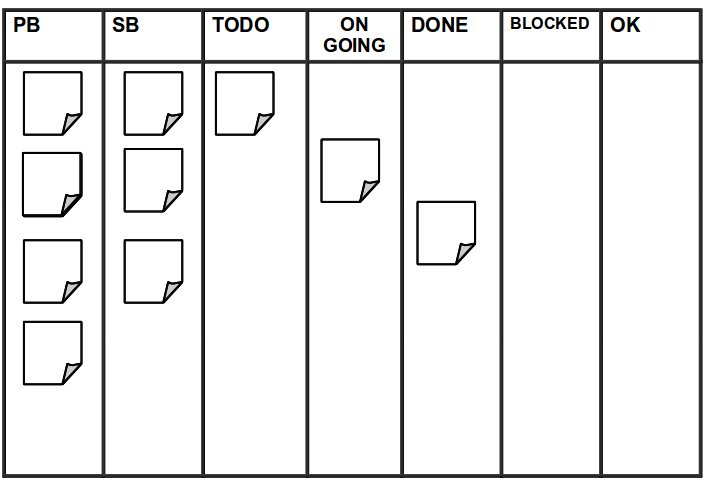
\includegraphics[width=0.9\textwidth]{ScrumKanbanBoard}
  \caption{Tablero Kanban para Scrum}
  \centering
  \label{fig:ScrumKanbanBoard} %\ref{fig:ScrumKanbanBoard}
\end{figure}

\subsubsection{Ejemplo de un Scrum board}

Un Scrum board, Kamban Board o taskboard físico (Ver figura \ref{fig:ScrumBoard}) es una tabla donde se colocan postick representando tareas.

\begin{figure}[h]
  \centering
  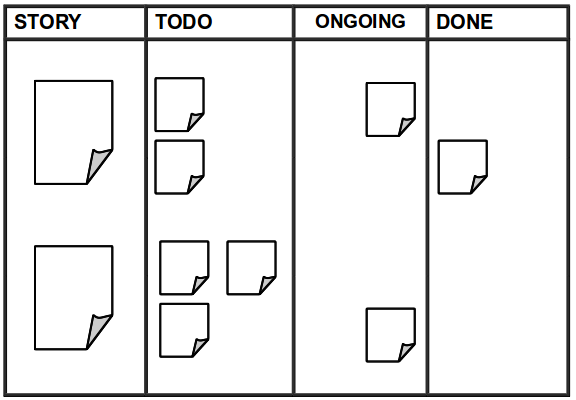
\includegraphics[width=0.8\textwidth]{ScrumBoard}
  \caption{Tablero Scrum}
  \centering
  \label{fig:ScrumBoard} %\ref{fig:ScrumBoard}
\end{figure}

\subsection{Gráficos de esfuerzo pendiente}

\subsubsection{Gráfico Burndown}
Un gráfico de trabajo pendiente o "Burndown charts" es uno que muestra el trabajo restante o que queda por hacer versus tiempo. Muestra la velocidad a la que se están completando los PBIs o historias reflejando el avance y permitiendo extrapolar si el Equipo podrá completar el trabajo en el tiempo restante.

Se pueden utilizan dos gráficos de esfuerzo pendiente:

\begin{enumerate}

\item \textbf{Burndown de Sprint:} Días u horas pendientes para completar las tareas de la iteración (sprint burndown chart), realizado a partir de la lista de tareas de la iteración. Normalmente se utiliza para saber cuánto falta para terminar las historias comprometidas en un Sprint. Es un diagrama de dos ejes: en el eje X el tiempo en días de duración del sprint, en el eje Y la cantidad de trabajo comprometida con el cliente durante el sprint en las unidades que se hayan acordado.

\item \textbf{Burndown de Proyecto:} Días pendientes para completar los requisitos del producto o proyecto (product burndown chart), realizado a partir de la lista de requisitos priorizada (Product Backlog).

\end{enumerate}

\subsubsection{Gráfico Burn-Up}

El gráfico Burn-up es muy similar al Burndown, con la diferencia de que se parte del cero, y se va marcando la cantidad de trabajo completado. En este gráfico la curva va hacia arriba asercándose a una línea que representa el alcance comprometido. En este tipo de gráfico es más fácil visualizar los cambios de alcance.

